
\documentclass{beamer}
\usetheme{ucl}

\usepackage[utf8]{inputenc}


%%% Increase the height of the banner: the argument is a scale factor >=1.0
%\setbeamertemplate{banner}[ucl][10.0]

%%% Change the colour of the main banner
%%% The background should be one of the UCL colours (except pink or white):
%%%   black,darkpurple,darkred,darkblue,darkgreen,darkbrown,richred,midred,
%%%   navyblue,midgreen,darkgrey,orange,brightblue,brightgreen,lightgrey,
%%%   lightpurple,yellow,lightblue,lightgreen,stone
\setbeamercolor{banner}{bg=darkpurple}
%\setbeamercolor{banner}{bg=yellow,fg=black}

%%% Add a stripe behind the banner
%\setbeamercolor{banner stripe}{bg=darkpurple,fg=black}

%%% The main structural elements
\setbeamercolor{structure}{fg=black}

%%% Author/Title/Date and slide number in the footline
\setbeamertemplate{footline}[author title date]

%%% Puts the section/subsection in the headline
% \setbeamertemplate{headline}[section]

%%% Puts a navigation bar on top of the banner
%%% For this to work correctly, the each \section command needs to be
%%% followed by a \subsection. Requires one extra compile.
% \setbeamertemplate{headline}[miniframes]
%%% Accepts an optional argument determining the width
% \setbeamertemplate{headline}[miniframes][0.3\paperwidth]


%%% Puts the frame title in the banner
%%% Won't work correctly with the above headline templates
%\useoutertheme{ucltitlebanner}
%%% Similar to above, but smaller (and puts subtitle on same line as title)
\useoutertheme[small]{ucltitlebanner}

%%% Gives block elements (theorems, examples) a border
% \useinnertheme{blockborder}
%%% Sets the body of block elements to be clear
% \setbeamercolor{block body}{bg=white,fg=black}

%%% Include CSML logo on title slide
%\titlegraphic{\includegraphics[width=0.16\paperwidth]{csml_logo}}

%%% Include CSML logo in bottom right corner of all slides
%\logo{\includegraphics[width=0.12\paperwidth]{csml_logo}}

%%% Set a background colour
% \setbeamercolor{background canvas}{bg=lightgrey}

%%% Set a background image
%%% Some sample images are available from the UCL image store:
%%%   https://www.imagestore.ucl.ac.uk/home/start
% \setbeamertemplate{background canvas}{%
%   \includegraphics[width=\paperwidth]{imagename}}



%%%%%% Some other settings that can make things look nicer
%%% Set a smaller indent for description environment
\setbeamersize{description width=2em}
%%% Remove nav symbols (and shift any logo down to corner)
\setbeamertemplate{navigation symbols}{\vspace{-2ex}}








\DeclareMathOperator{\Cov}{Cov}
\DeclareMathOperator{\Var}{Var}
\DeclareMathOperator{\E}{\mathbb{E}}
\DeclareMathOperator{\Proba}{\mathbb{P}}

\newcommand{\Covb}[2]{\ensuremath{\Cov\!\left[#1,#2\right]}}
\newcommand{\Eb}[1]{\ensuremath{\E\!\left[#1\right]}}
\newcommand{\Pb}[1]{\ensuremath{\Proba\!\left[#1\right]}}
\newcommand{\Varb}[1]{\ensuremath{\Var\!\left[#1\right]}}

% norm
\newcommand{\norm}[1]{\| #1 \|}

\newcommand{\indep}{\rotatebox[origin=c]{90}{$\models$}}





\usepackage{mathptmx,amsmath,amssymb,graphicx,bibentry,bbm,ragged2e}
\usepackage[english]{babel}

\makeatletter

\newcommand{\noun}[1]{\textsc{#1}}
\newcommand{\jitem}[1]{\item \begin{justify} #1 \end{justify} \vfill{}}
\newcommand{\sframe}[2]{\frame{\frametitle{#1} #2}}

\newenvironment{centercolumns}{\begin{columns}[c]}{\end{columns}}
%\newenvironment{jitem}{\begin{justify}\begin{itemize}}{\end{itemize}\end{justify}}



%\usetheme{Warsaw}
%\setbeamertemplate{footline}[text line]{}
%\setbeamertemplate{headline}{}
%\setbeamercolor{structure}{fg=purple!50!blue, bg=purple!50!blue}

%\setbeamersize{text margin left=15pt,text margin right=15pt}

%\setbeamercovered{transparent}


\@ifundefined{showcaptionsetup}{}{%
 \PassOptionsToPackage{caption=false}{subfig}}
\usepackage{subfig}

\usepackage[utf8]{inputenc}
\usepackage[T1]{fontenc}

\usepackage{multirow}


\makeatother

\def \draft {1}

\usepackage{xparse}
\usepackage{ifthen}
\DeclareDocumentCommand{\comment}{m o o o o}
{\ifthenelse{\draft=1}{
    \textcolor{red}{\textbf{C : }#1}
    \IfValueT{#2}{\textcolor{blue}{\textbf{A1 : }#2}}
    \IfValueT{#3}{\textcolor{ForestGreen}{\textbf{A2 : }#3}}
    \IfValueT{#4}{\textcolor{red!50!blue}{\textbf{A3 : }#4}}
    \IfValueT{#5}{\textcolor{Aquamarine}{\textbf{A4 : }#5}}
 }{}
}
\newcommand{\todo}[1]{
\ifthenelse{\draft=1}{\textcolor{red!50!blue}{\textbf{TODO : \textit{#1}}}}{}
}




\begin{document}


\title[Building simulation models]{Building simulation models coupling territorial and network dynamics at the interface of disciplines and scales}

\author[J.~Raimbault]{J.~Raimbault$^{1,2,3\ast}$\\
\texttt{j.raimbault@ucl.ac.uk}
}


\institute[UCL]{$^{1}$CASA, UCL\\
$^{2}$UPS CNRS 3611 Complex Systems Institute Paris\\
$^{3}$UMR CNRS 8504 G{\'e}ographie-cit{\'e}s
}


\date[10/06/2021]{Spatial Data Science 2020\\
June 10th 2021
}

\frame{\maketitle}

% Keywords: Transportation Networks; Territorial Systems; Co-evolution; Simulation Models


\sframe{Interactions between networks and territories}{

% Interactions between transportation networks and the dynamics of land-use are crucial to take into account when planning and managing sustainable urban environments.

\justify

\begin{center}
\includegraphics[width=0.45\linewidth]{figures/accessp_withbridge_prd_EN.png}
\hspace{0.1cm}
\includegraphics[width=0.52\linewidth]{figures/avgaccess_facet.png}

\end{center}

\medskip


\textit{Accessibility as part of complex processes of co-evolution between transportation networks and territories.}

\medskip

\tiny

Raimbault, J. (2019). Evolving accessibility landscapes: mutations of transportation networks in China. In Aveline-Dubach, N., ed. \textit{Pathways of sustainable urban development across China - the cases of Hangzhou, Datong and Zhuhai}, pp 89-108. Imago. ISBN:978-88-94384-71-0

\nocite{raimbault:halshs-02265423}

}



\sframe{Literature mapping}{

% A quantitative understanding of such processes using models has been proposed by several disciplines, including Land-use Transport Interaction models or economic models of transport network growth.

\textit{Interdisciplinarity and interactions between networks and territories}

\medskip

%\vspace{-1cm}
\begin{center}
	\includegraphics[width=0.9\textwidth,trim={0 0 0 8cm},clip]{figures/2-2-2-fig-quantepistemo-citnw.jpg}	
\end{center}

\medskip

\tiny

\vspace{-1cm}

Raimbault, J. (2019). Exploration of an interdisciplinary scientific landscape. Scientometrics, 119(2), 617-641.

\nocite{raimbault2019exploration}

\medskip

Raimbault, J. (2021). An interdisciplinary bibliometric analysis of models for land-use and transport interactions. arXiv preprint arXiv:2102.13501.

\nocite{raimbault2021interdisciplinary}

}


\sframe{Defining co-evolution}{

% A co-evolution approach (in terms of circular causal relations) to modelling interactions between transportation networks and territories can be proposed, to simulate the dynamics of territories on long time scales. Such a viewpoint has however not been extensively explored, as the question is by nature interdisciplinary and at the interface of spatial and temporal scales.
% The purpose of this communication is to synthesise results obtained with simple agent-based and simulation models at different scales and integrating paradigms from different disciplines, from planning to transport geography, urban geography, physics and economics. These models have the common feature of strongly coupling territorial and transportation network dynamics.


\footnotesize
 
\textbf{Theoretical context:} 

  
\begin{itemize}
  \item Cities and territories understood from the viewpoint of Pumain's \textit{Evolutionary Urban Theory} \cite{pumain1997pour}
  \item Transportation networks materialising ``transactional projects'', following the \textit{Territorial Theory of Networks} \cite{dupuy1987vers}
\end{itemize}
 
\medskip


\textbf{Processes:} \textit{A multi-level definition of co-evolution:} 
\begin{enumerate}
	\item \textcolor{blue}{level of agents}
	\item \textcolor{green}{statistical level of agent populations (niches)}
	\item \textcolor{red}{global system level}
\end{enumerate}  


\medskip


\textbf{Corresponding approaches: }

\begin{enumerate}
	\item \textcolor{blue}{Empirical (microscopic level)}
	\item \textcolor{green}{Modeling morphogenesis (niche level)}
	\item \textcolor{red}{Urban dynamics models (macroscopic level)}
\end{enumerate}

\medskip

\tiny

Raimbault, J. (2018). Caract{\'e}risation et mod{\'e}lisation de la co-{\'e}volution des r{\'e}seaux de transport et des territoires (Doctoral dissertation, Universit{\'e} Paris 7 Denis Diderot).

\nocite{raimbault2018caracterisation}

\smallskip

Raimbault, J. (2019). Modeling interactions between transportation networks and territories: a co-evolution approach. arXiv preprint arXiv:1902.04802.

\nocite{raimbault2019modelingsynth}

}

\sframe{Characterising co-evolution}{


\begin{center}
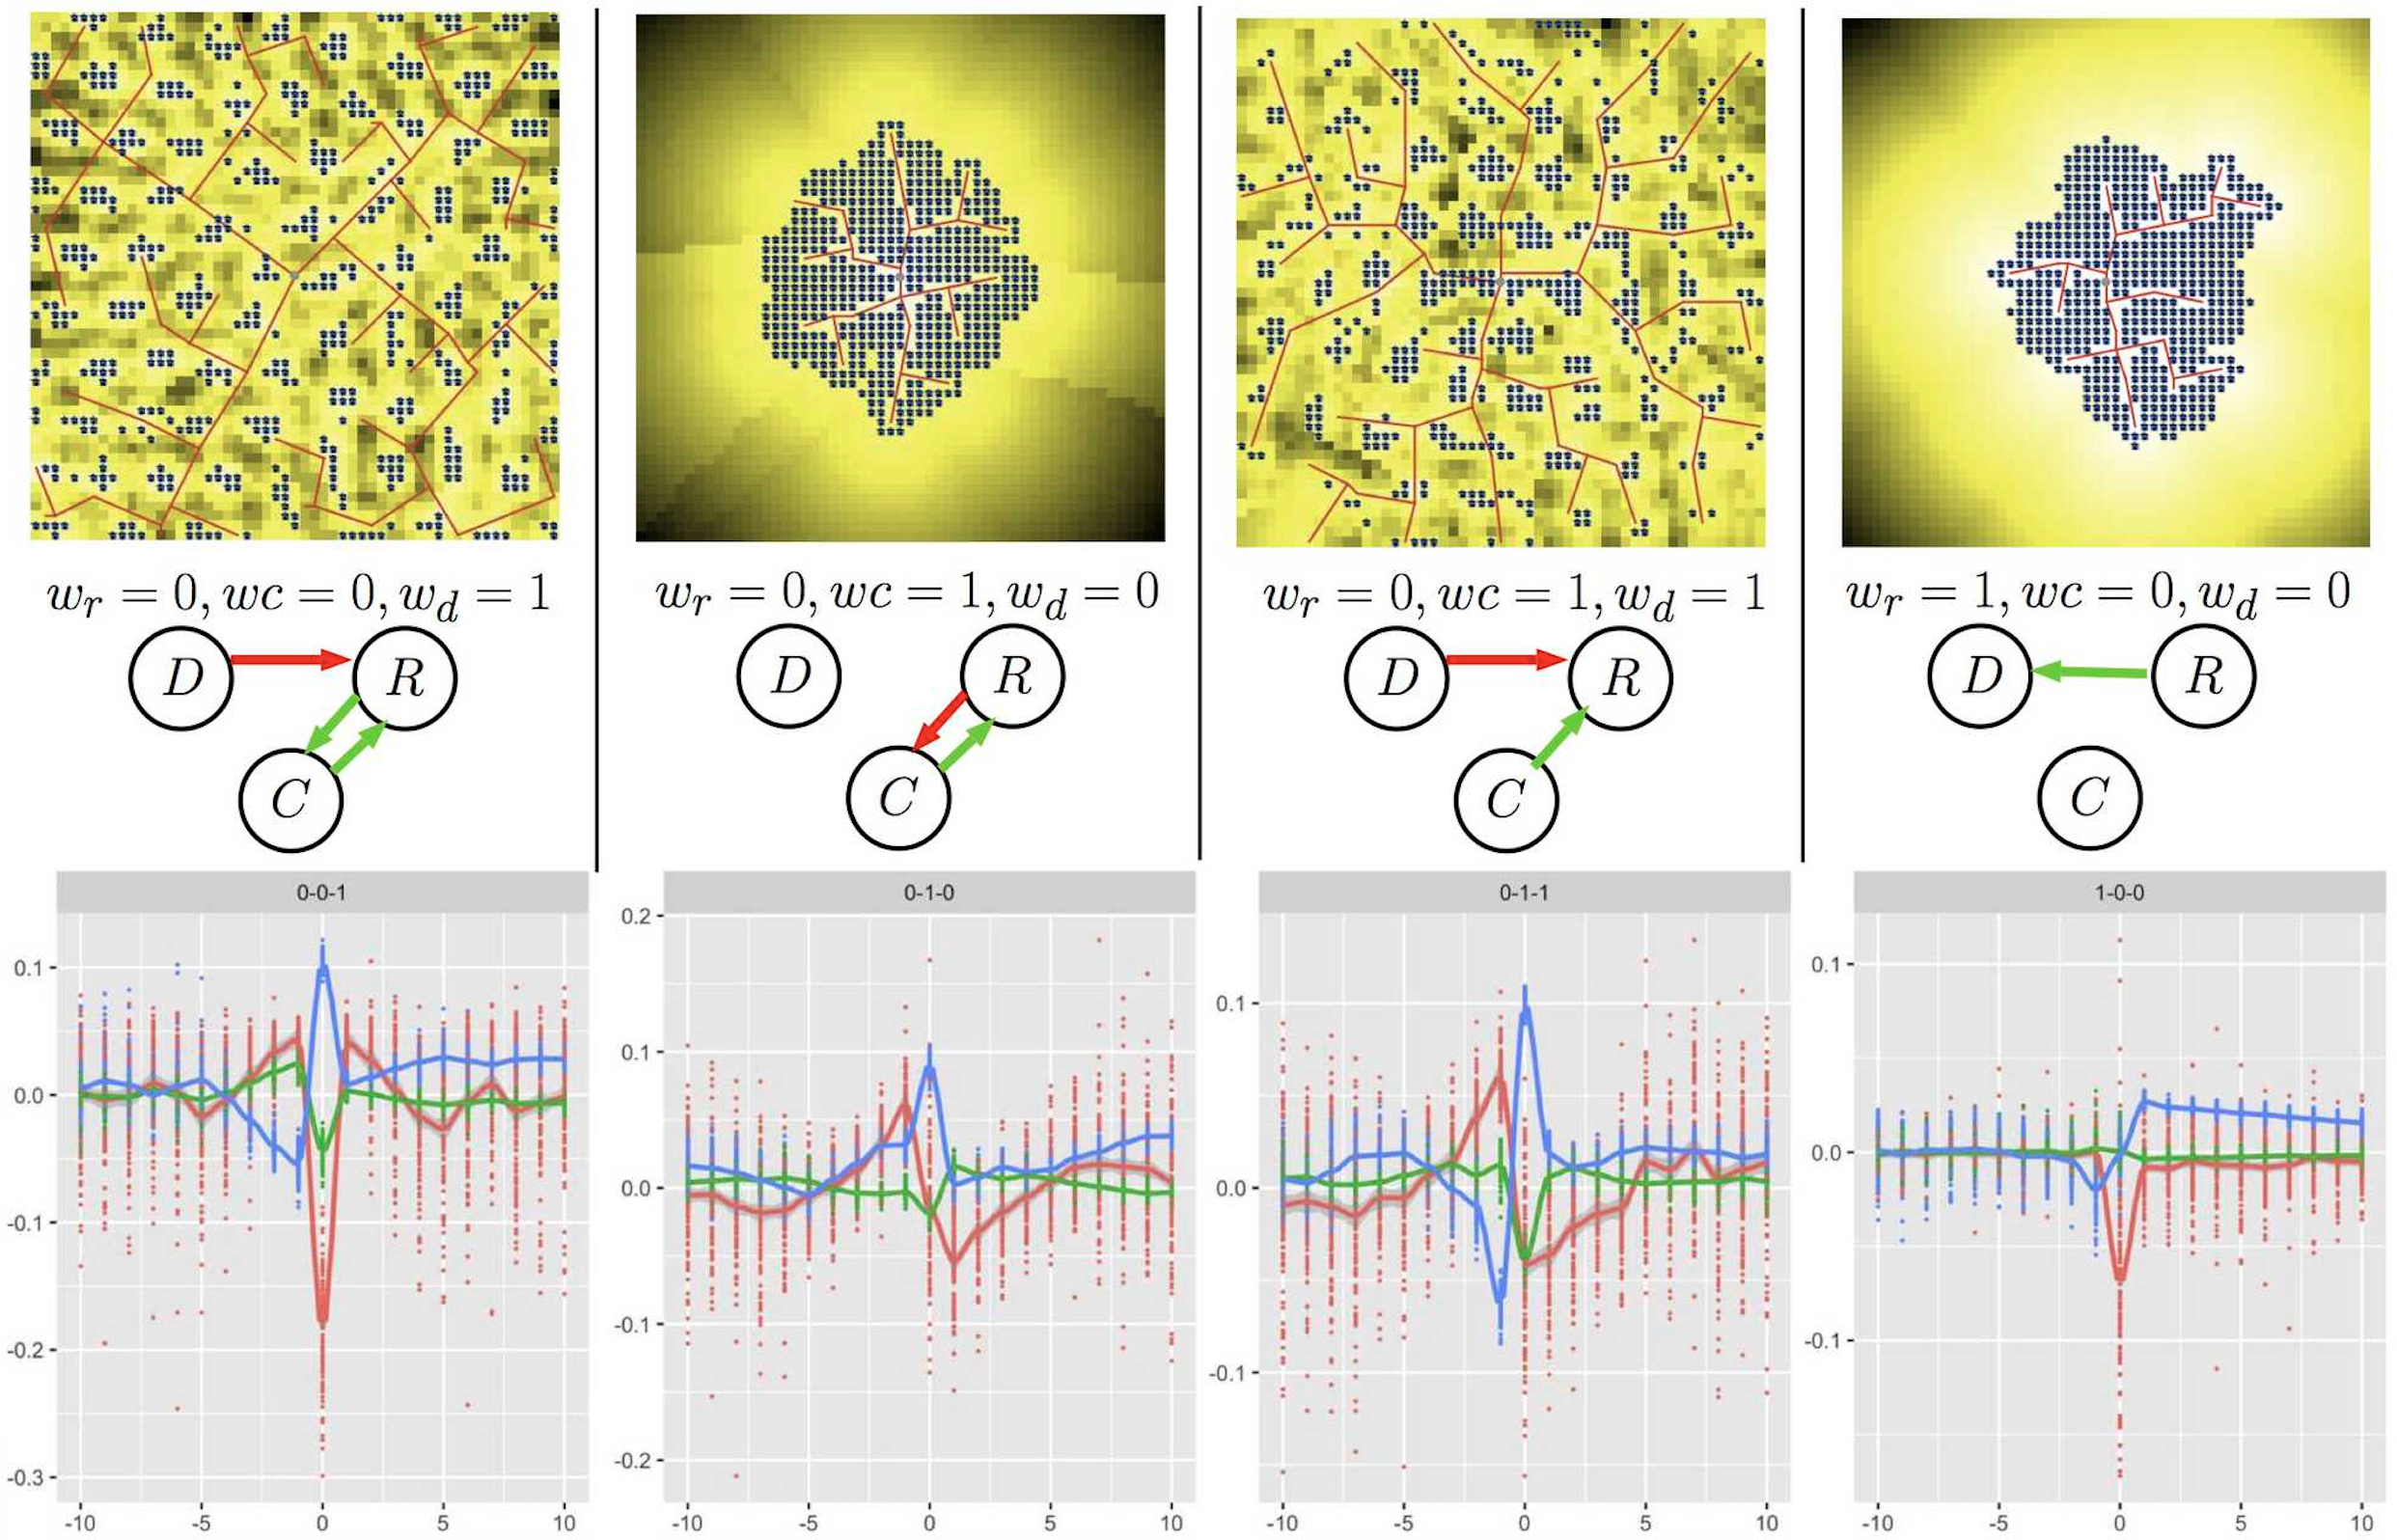
\includegraphics[width=0.85\linewidth]{figures/carac_regimes_1.png}
\end{center}

\medskip

\tiny


Raimbault, J., Banos, A., \& Doursat, R. (2014). A Hybrid Network/Grid Model of Urban Morphogenesis and Optimization. In 4th International Conference on Complex Systems and Applications (pp. 51-60).

\nocite{raimbault2014hybrid}

\smallskip

Raimbault, J. (2017). Identification de causalit{\'e}s dans des donn{\'e}es spatio-temporelles. In Spatial Analysis and GEOmatics 2017.

\nocite{raimbault2017identification}

}



\sframe{Mesoscopic scale: morphogenesis models}{

%A first model at the scale of the urban area explores the coupling between a population density generation model based on aggregation-diffusion processes with multiple network growth heuristics. This co-evolution model capture in practice the growth of urban form, and multiple dynamical regimes between population and road networks. It is calibrated on empirical morphological and network measures computed on spatial windows covering Europe.

\begin{center}
\includegraphics[width=0.8\linewidth]{figures/meso_multimodeling.png}
\end{center}

\medskip

\tiny

Raimbault, J. (2018). Multi-modeling the morphogenesis of transportation networks. In Artificial Life Conference Proceedings (pp. 382-383). MIT Press, Cambridge.

\nocite{raimbault2018multi}

}


\sframe{Morphogenesis models}{



\footnotesize

\justify
\textit{A morphogenesis model with reaction-diffusion and multi-modeling of network growth: complementarity of heuristics, calibration for Europe on forms and their correlations}

\smallskip

\begin{center}
\includegraphics[width=0.25\linewidth,height=0.6\textheight]{figures/meso-nwgrowth.png}
\includegraphics[width=0.6\linewidth,height=0.6\textheight]{figures/meso-calib.jpg}
\end{center}


\smallskip

\tiny

Raimbault, J. (2018). Calibration of a density-based model of urban morphogenesis. PloS one, 13(9), e0203516.

\nocite{raimbault2018calibration}

\smallskip

Raimbault, J. (2019). An urban morphogenesis model capturing interactions between networks and territories. In The Mathematics of Urban Morphology (pp. 383-409). Birkhäuser, Cham.

\nocite{raimbault2019urban}

}







\sframe{Macroscopic interaction models}{


% We then develop a family of models at the macroscopic scale to simulate systems of cities, and more particularly the co-evolution of cities and interurban transportation networks. Building on dynamical models developed in the frame of Pumain's evolutionary urban theory, this allows investigating self-reinforcement processes between urban and network hierarchies. We show in particular that these models are effectively capturing a diversity of co-evolution regimes (in the sense of a circular causation) between the properties of network and cities.


\textit{System of cities interaction model including network evolution; production of multiple co-evolution regimes and calibration for France.}

\medskip

\includegraphics[width=0.6\textwidth]{figures/macrocoevol_en.png}
\includegraphics[width=0.39\linewidth]{figures/6-2-2-fig-macrocoevol-correlations.jpg}


\bigskip

\tiny

Raimbault, J. (2020). Indirect evidence of network effects in a system of cities. Environment and Planning B: Urban Analytics and City Science, 47(1), 138-155.

\nocite{raimbault2020indirect}

\smallskip

Raimbault, J. (2021). Modeling the co-evolution of cities and networks. In Niel, Z., Rozenblat, C., eds. \textit{Handbook of Cities and Networks}, Edwar Elgar Publishing, \textit{in press}.

\nocite{raimbault2021modeling}

}


\sframe{Capturing co-evolution at the macro scale}{

% slide on simpopnet exploration

\textit{Similar models for co-evolution capturing it only partly.}

\medskip

\begin{center}
\includegraphics[width=0.37\textwidth]{figures/Simpopnet_Fig1.png}\hspace{0.3cm}
\includegraphics[width=0.57\textwidth]{figures/Simpopnet_Fig4.png}
\end{center}

\medskip
\tiny

Raimbault, J. (2020). Unveiling co-evolutionary patterns in systems of cities: a systematic exploration of the simpopnet model. In Theories and Models of Urbanization (pp. 261-278). Springer, Cham.

\nocite{raimbault2020unveiling}

}



\sframe{Extending LUTI models: transport governance}{

% We finally describe an agent-based model at the metropolitan scale including more complex mechanisms for coupling, in particular a governance process for the growth of the transport network based on game theory, coupled to a Lowry model for land-use dynamics. This model is applied and calibrated on the case study of Pearl River Delta, China.

\textit{A co-evolution model integrating transport governance dynamics through game theory}

\medskip

\begin{center}
\includegraphics[width=0.58\textwidth]{figures/Lutecia_Fig1.png}\hspace{0.2cm}
\includegraphics[width=0.35\textwidth]{figures/7-3-3-fig-lutecia-governance.jpg}
\end{center}

\medskip

\tiny

Raimbault, J. \& Le N{\'e}chet F. (2021, forthcoming). Introducing endogenous transport provision in a LUTI model to explore polycentric governance systems. Journal of Transport Geography.

\nocite{raimbault2021introducing}

}





\sframe{Towards multi-scale models}{


\textit{Processes specific to scales, models across scales require dedicated ontologies}


\bigskip

\begin{center}
	\includegraphics[width=0.9\textwidth]{figures/multiscale_morph.pdf}
\end{center}

\nocite{raimbault2021strong}

\tiny

Raimbault, J. (2021). Strong coupling between scales in a multi-scalar model of urban dynamics. arXiv preprint arXiv:2101.12725.

}


\sframe{Model exploration methods to foster knowledge integration}{
	
	% This synthesis emphasises the role of simulation models in the production of knowledge. Indeed, most results are obtained through the systematic exploration of models and the application of new model validation methods provided by the OpenMOLE platform.
	
	OpenMOLE software \cite{reuillon2013openmole}: \textit{(i) Innovative exploration methods; (ii) Scaling of methods on high performance computing environments; (iii) Scripts to embed and couple models.}
	
	\smallskip
	
	\centering
	
	\includegraphics[width=0.8\textwidth]{figures/openmoleGal.png}
	
}




\sframe{Validation: spatial sensitivity analysis}{

% Such systematic explorations enable the testing of hypothesis, and clarify theory building when linked to empirical data and stylised facts.

\centering

\includegraphics[width=0.95\linewidth]{figures/spatial_sa.png}

\nocite{raimbault2019second}
\nocite{raimbault2019generating}
\nocite{raimbault2019space}
\nocite{raimbault2020scala}

}









\sframe{Conclusion}{

%  This also facilitates a modular approach to modeling, and thus the coupling of concepts and processes from different disciplines.


\justify

$\rightarrow$ Multiple dimensions of urban systems: \textbf{models at the interface of disciplines.}

\medskip

$\rightarrow$ Multiple scales: \textbf{at the interface of scales.}

\medskip

$\rightarrow$ Multiple types of knowledge: \textbf{simulation models and their exploration and validation as an integrating approach.}


\bigskip
\bigskip
\bigskip

\textbf{To use OpenMOLE (free and open software) and contribute: }\\
\url{https://openmole.org}

\bigskip

\textbf{All models open source at }

\url{https://github.com/JusteRaimbault/CityNetwork}




}






%%%%%%%%%%%%%%%%%%%%%
\begin{frame}[allowframebreaks]
\frametitle{References}
\bibliographystyle{apalike}
\bibliography{biblio}
\end{frame}
%%%%%%%%%%%%%%%%%%%%%%%%%%%%










\end{document}















